\section{Experiments}
\label{sec:experiments}

% introduceer experimenten?
For all experiments, the model was trained on the training split of the MSCOCO dataset. Captions were transcribed phonetically automatically using eSpeak. Stress and pause markers were cleaned out, as well as word boundaries, leaving only the phonemic symbols. % Visual input consisted of  ja wat eigenlijk. misschien moet dit wel in de models-sectie?
\subsection{Prediction of visual features}
\label{subsec:visual}
The models are trained and evaluated on the prediction of visual
feature vectors from captions. While our goal is not to develop an
image retrieval method, we use this this task as it reflects the ability to extract visually salient semantic information from language.
For the experiments on the prediction of visual features all models
were trained on the training set of MS COCO. As validation and test data we
used a random sample of 5000 images each from the MS COCO validation set. 

Figure~\ref{fig:loss} shows the value of the validation average cosine distance
between the predicted visual vector and the target vector for three
random initializations of each of the model types. 

The Phonetic GRU model is more sensitive to the initialization: one
can clearly distinguish three separate trajectories. The word-level models
are much less affected by random initialization. In terms of the
overall performance, the {\sc Phon GRU} model falls between the
{\sc Word Sum} model and the {\sc Word GRU} model.

\begin{figure}
    \centering
  \begin{minipage}{0.45\textwidth}
    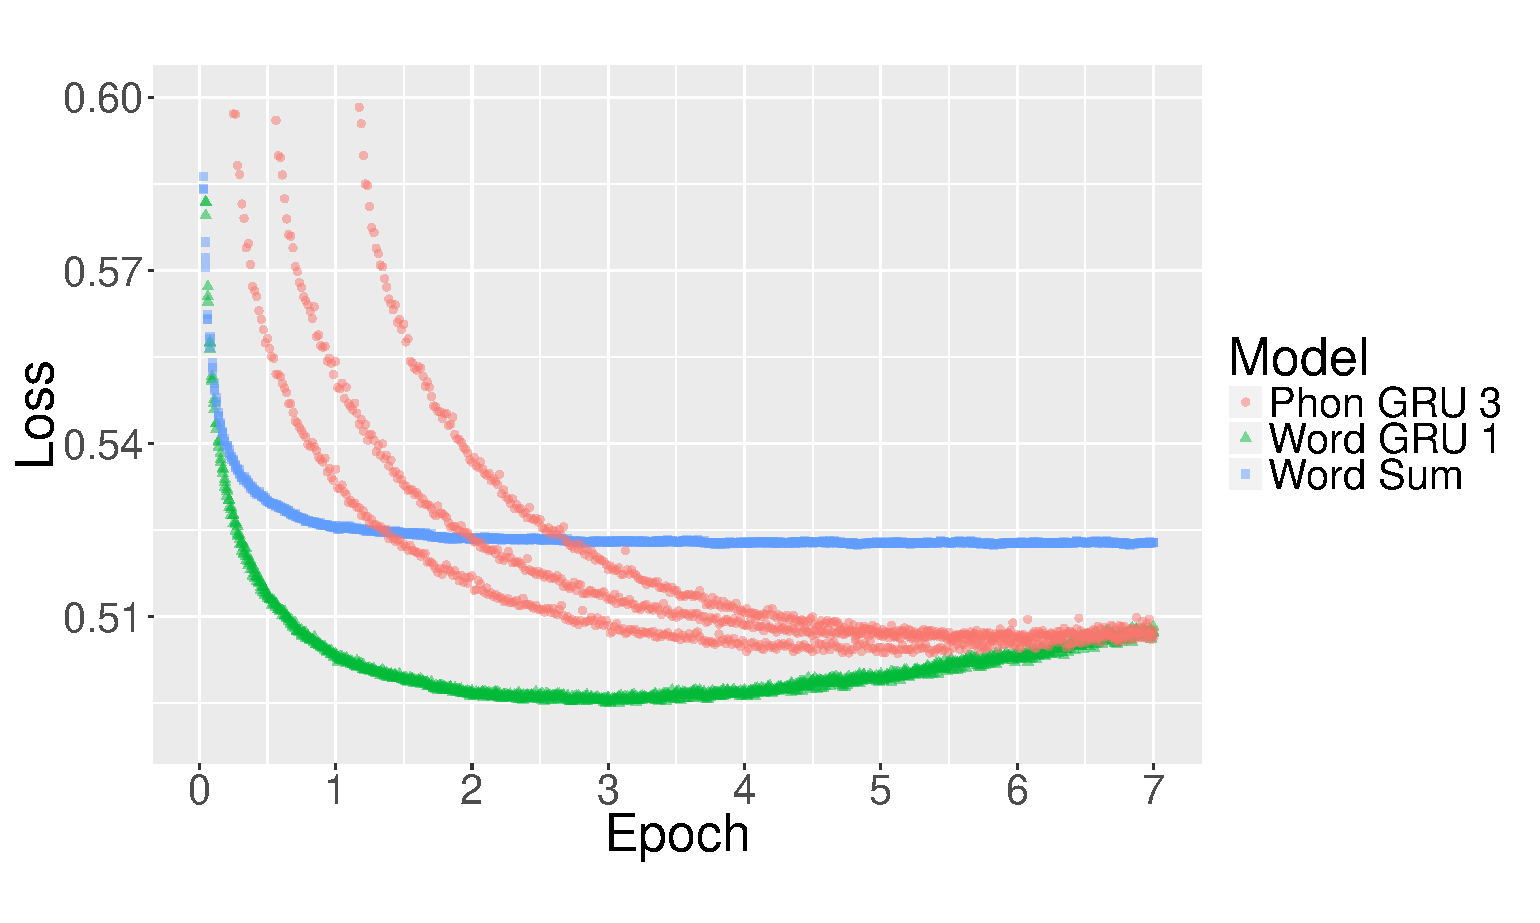
\includegraphics[scale=0.32]{loss-zoom.pdf}
    \caption{Value of the loss function on validation data during
      training. Three random initialization of each model are shown.}
    \label{fig:loss}
  \end{minipage}
\hspace{0.3cm}
  \begin{minipage}{0.45\textwidth}
    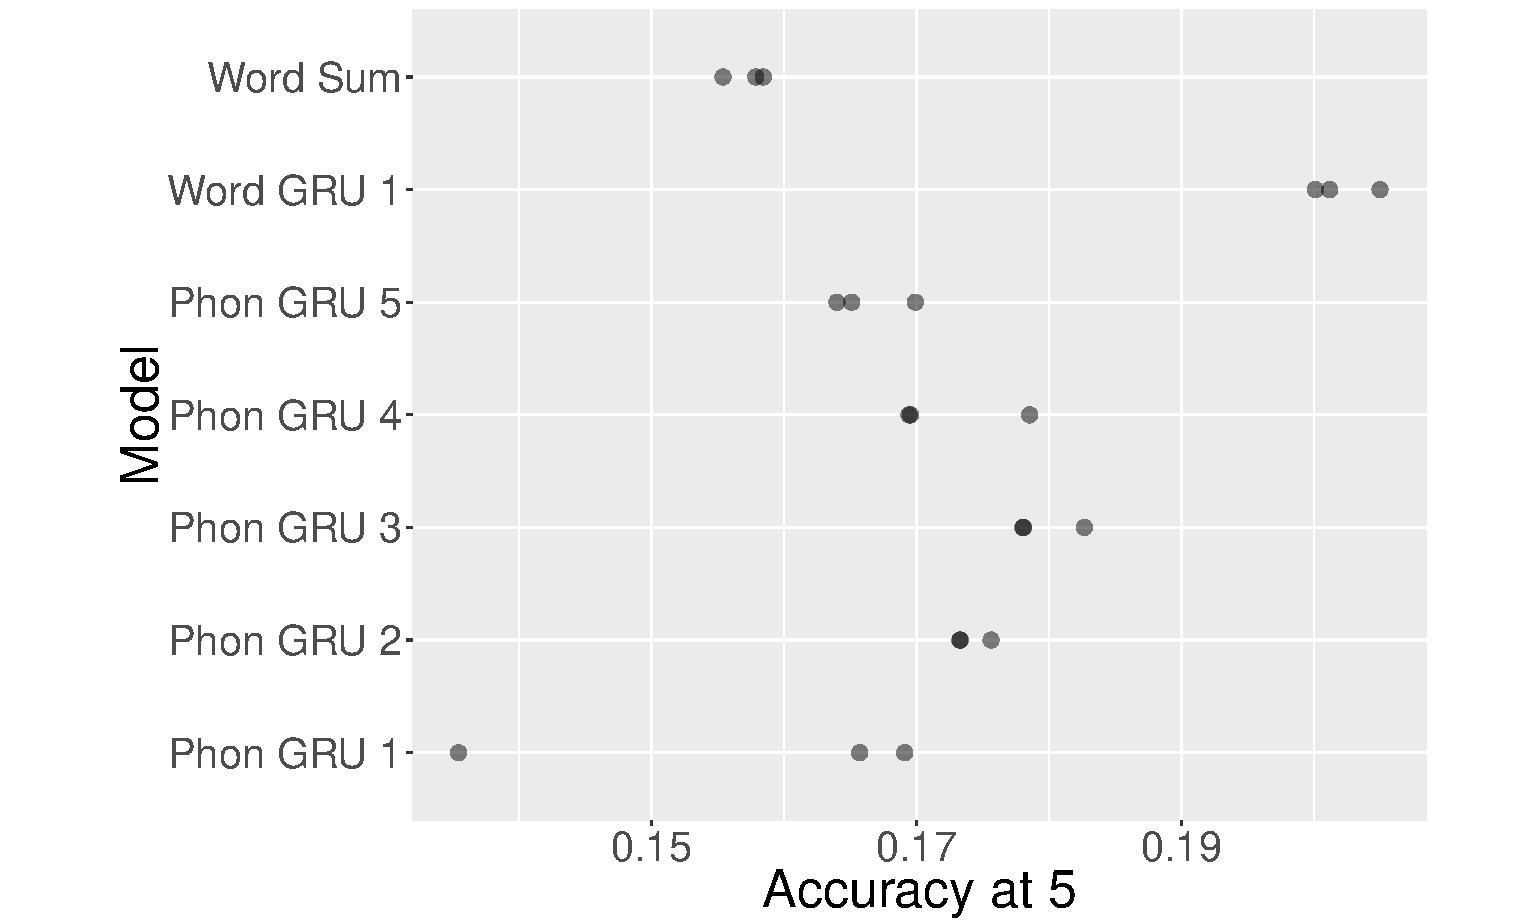
\includegraphics[scale=0.32]{accat5.pdf}
    \caption{Validation accuracy at 5 on the image retrieval task.}
    \label{fig:accat5}
  \end{minipage}
\end{figure}

We also evaluated the models on how well they perform when used to
search images: for each validation sentence the model was used to predict the
visual vector. The image vectors in the validation data were then
ranked by cosine similarity to the predicted vector, and the
proportion of times the correct image was among the top 5 was
reported. By {\it correct} image we mean the one which the sentence
was used to describe (even though often many other images are also
good matches to the sentence). 

In Figure~\ref{fig:accat5} we report the validation accuracies on this
task for the two word-level models, as well as for the Phon GRU
model with different number of hidden layers. We trained each model
version with three random initializations for each model setting, and
evaluate after each epoch. We report the score of the best epoch for
each initialization. 
The overall ranking of the models matches the direct
evaluation of the loss function above: the phoneme-level models are in
between the two word-level models. {\sc Phon GRU} with three
hidden layers is the best of the phoneme-level models.

In Table~\ref{tab:accat5test} we show the accuracies of the best
version of each of the models types on the test images; these are also
the model versions used in all subsequent experiments. The accuracy @
5 for the {\sc Word GRU} is comparable to what
\newcite{chrupala2015learning} report for their multitask {\sc
  Imaginet} model, whose visual pathway has the same
structure. \newcite{vendrov2015order} report substantially higher
scores for image search with a word level GRU model, with the
following main differences from our setting: better image features,
larger training set, and a loss function optimized for the ranking
task.\footnote{We have preliminary results indicating that most of the
  analyses in the rest of Section~\ref{sec:experiments} show the same general
  pattern for phoneme models trained following the setting of
  \newcite{vendrov2015order}.}.

% \begin{table}
%   \centering
%   \begin{tabular}{ll|r}
%  Model     & Layers & Acc. at 5 \\\hline
%  Word Sum  & 0      & 0.158 \\
%  Word GRU  & 1      & 0.205 \\\hline
%  Phon GRU  & 1      & 0.169  \\
%  Phon GRU  & 2      & 0.176  \\
%  Phon GRU  & 3      & \bf 0.183  \\  
%  Phon GRU  & 4      & 0.179 \\
%  Phon GRU  & 5      & 0.170 \\
%   \end{tabular}
% \caption{Accuracy at 5 on the image retrieval task.}
% \label{tab:accat5}
% \end{table}

\subsection{Word boundary prediction}
To explore the sensitivity of the model to linguistic structure at the sub-word level, we trained logistic regression models to predict and recognize word boundaries from the activation patterns of all hidden layers. The task of the prediction models was to determine whether a certain timestep was a word end, given the activation pattern at one of the hidden layers. The task of the recognition models was to identify word onsets based on activation patterns. Data was shuffled before training and testing. All models were trained on a random selection of 5000 sentences from the validation split, and tested on the rest of the validation split. % model settings %are these standardized splits? (no) By whom? how much is 'the rest'? was it a good idea to randomly select sentences, rather than pictures?
For comparison, we also trained logistic regression models on n-gram data to perform the same tasks. The features available to these models were positional n-grams. %write more once you know what you're doing

\subsection{Word Similarity} % you may want to say semantic, although that is somewhat questionable, and relatedness rather than similarity...
To understand the encoding of semantic information by the model, we compared similarity of activation vectors to human similarity judgements from the MEN dataset. %cite 
For each word pair in the MEN dataset, the words were transcribed phonetically automatically and then fed to the model individually. Cosine similarity between the activation patterns of the third hidden layer at the last timestep was taken as the measure of similarity. % did you take the last timestep or end-of-sentence-symbol? If last timstep, why?
Since the model has access to the surface forms of words, it may be able to exploit surface similarity when determining semantic relatedness. This may especially be the case when encountering infrequent words. If the meaning of a word is not known from previous encounters, well-known words that are similar in form may provide some clue to its meaning. To determine whether such an effect of phonetic similarity exists, a measure of phonemic difference was included: the edit distance between the phonetic transcriptions of the two words, normalized by dividing it by the length of the longest transcription.

\subsection{Word similarity: replacement}
The experiment previously described takes cosine similarity between the activations of the last hidden layer as a measure of word similarity, in analogy to how similarity of word embeddings is commonly quantified. However, the last hidden layer of our model is very different to an embedding layer. Its task is to integrate information over a whole sentence, as a basis for predicting features of the visual scene it describes. In the current experiment, the difference between two words is how much the prediction of the visual scene changes when one word replaces the other. % niet waar je pakt de laatste hidden layer, niet de uiteindelijke voorspelling
The input data were sentences from the validation part %je hebt nu train-part! OPNIEUW 
of the MSCOCO dataset that contained either one of the two words of each word pair in the MEN dataset. In each of these sentences % niet waar, je neemt er max 20. also de laatste zin was onontwarbaar
the word that got it selected, was replaced by its counterpart from the MEN dataset. The resulting sentence was transcribed phonetically. Similarity of the sentences was measured by taking the cosine similarity between the activation vector of the highest hidden layer at the end-of-sentence symbol for the original sentence and the sentence in which the original word had been replaced. The similarity score of a word pair was the average similarity of the sentence pairs. % something about this perhaps not being simmetric? 
